\documentclass{beamer}

\usepackage{hyperref}       % For clickable hyperlinks.
\usepackage{booktabs}
\usepackage{cprotect}
\usepackage{amsmath}
\usepackage{hologo}
\usepackage{fancyvrb}       % Fancy verbatim environments.
\newenvironment{CVerbatim} % Verbatim environment with centered text.
{\VerbatimEnvironment\begin{center}\begin{BVerbatim}}{\end{BVerbatim}\end{center}}

\usepackage{pgfplots}
\pgfplotsset{width=5cm,compat=1.18}
\usepackage{tikz}
\usepackage[linguistics]{forest}
\forestset{
  nice nodes/.style={
    for tree={
      inner sep=0pt,
      fit=band,
    },
  },
  default preamble=nice nodes,
}

%easy traces with subscript (from Pomona LaTeX guide)
\newcommand{\tr}[1]{\textit{t}\textsubscript{\textit{#1}}}

\usepackage{fontspec}
\newfontfamily{\brillfam}{Brill}
\newcommand{\brill}[1]{{\brillfam{}#1}}

\newfontfamily{\arial}{Arial}
\newfontfamily{\bettertimes}{Times New Roman}
\newfontfamily{\comic}{Comic Sans MS}
\newfontfamily{\minya}[
    Path            =   ./fonts/minya-nouvelle/,
    BoldFont        =   Minya-Nouvelle-Bd.otf,
    ItalicFont      =   Minya-Nouvelle-It.otf,
    BoldItalicFont  =   Minya-Nouvelle-Bd-It.otf]{Minya-Nouvelle-Rg.otf}

\usepackage[backend=biber, style=apa]{biblatex}
\addbibresource{bib.bib}

\newcommand{\code}[1]{\texttt{#1}}
\newcommand{\filename}[1]{\texttt{#1}}
\newcommand{\switch}[1]{\texttt{\textbackslash#1}}
\newcommand{\command}[2]{\texttt{\textbackslash#1\{#2\}}}
\newcommand{\optcommand}[2]{\texttt{\textbackslash#1[#2]}}
\newcommand{\commandopt}[3]{\texttt{\textbackslash#1[#3]\{#2\}}}
\newcommand{\latexenv}[1]{\texttt{\textbackslash{}begin\{#1\}}\ldots\texttt{\textbackslash{}end\{#1\}}}

\newcommand{\red}[1]{\textcolor{red}{#1}}
\newcommand{\blue}[1]{\textcolor{blue}{#1}}
\newcommand{\green}[1]{\textcolor{green}{#1}}
\newcommand{\purple}[1]{\textcolor{purple}{#1}}

\AtBeginSection[]
{
    \begin{frame}
        \frametitle{Table of Contents}
        \tableofcontents[currentsection]
    \end{frame}
}

\usetheme{Frankfurt}

\title{\LaTeX{} for the Humanities}
\subtitle{A short introduction}
\author{Dr.\ Xander Vertegaal}
\institute{Utrecht University Centre for Digital Humanities}
\date{February 28, 2024}

\begin{document}

\begin{frame}
    \titlepage
\end{frame}

\begin{frame}{Table of Contents}
    \tableofcontents
\end{frame}

\section{Introduction}

\begin{frame}{What is \LaTeX?}
    \begin{columns}
        \begin{column}{0.6\textwidth}
            \begin{itemize}
                \item<1-> \TeX{} (Donald Knuth, 1978)
                \item<1-> Name < Greek \brill{τέχνη} \emph{techne} (`art', `craft')
                \item<2-> A \emph{compiler} turns your text and commands into a PDF.
                \item<3-> Original \TeX{} is rather complicated.
                \item<4-> \LaTeX{} (Leslie Lamport, 1984)
                \item<4-> Macro package for \TeX{}
            \end{itemize}
        \end{column}
        \begin{column}{0.4\textwidth}
            \begin{figure}[h]
                \only<1>{
                    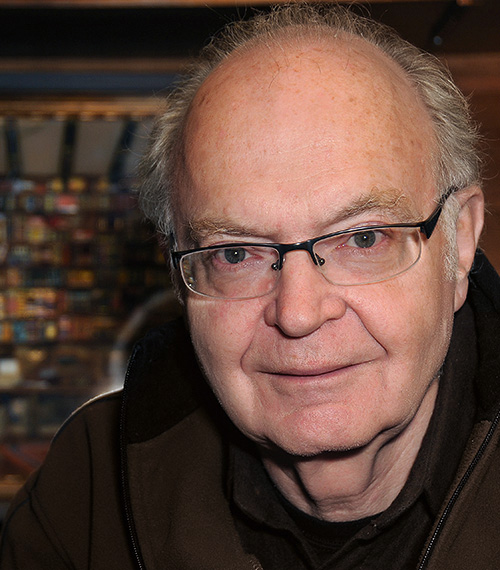
\includegraphics[scale=0.2]{./assets/knuth.jpg}
                    \caption{Donald Knuth}
                }
                \only<2>{
                    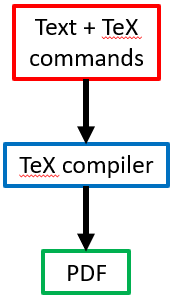
\includegraphics[scale=0.6]{./assets/compiler.png}
                }
                \only<4>{
                    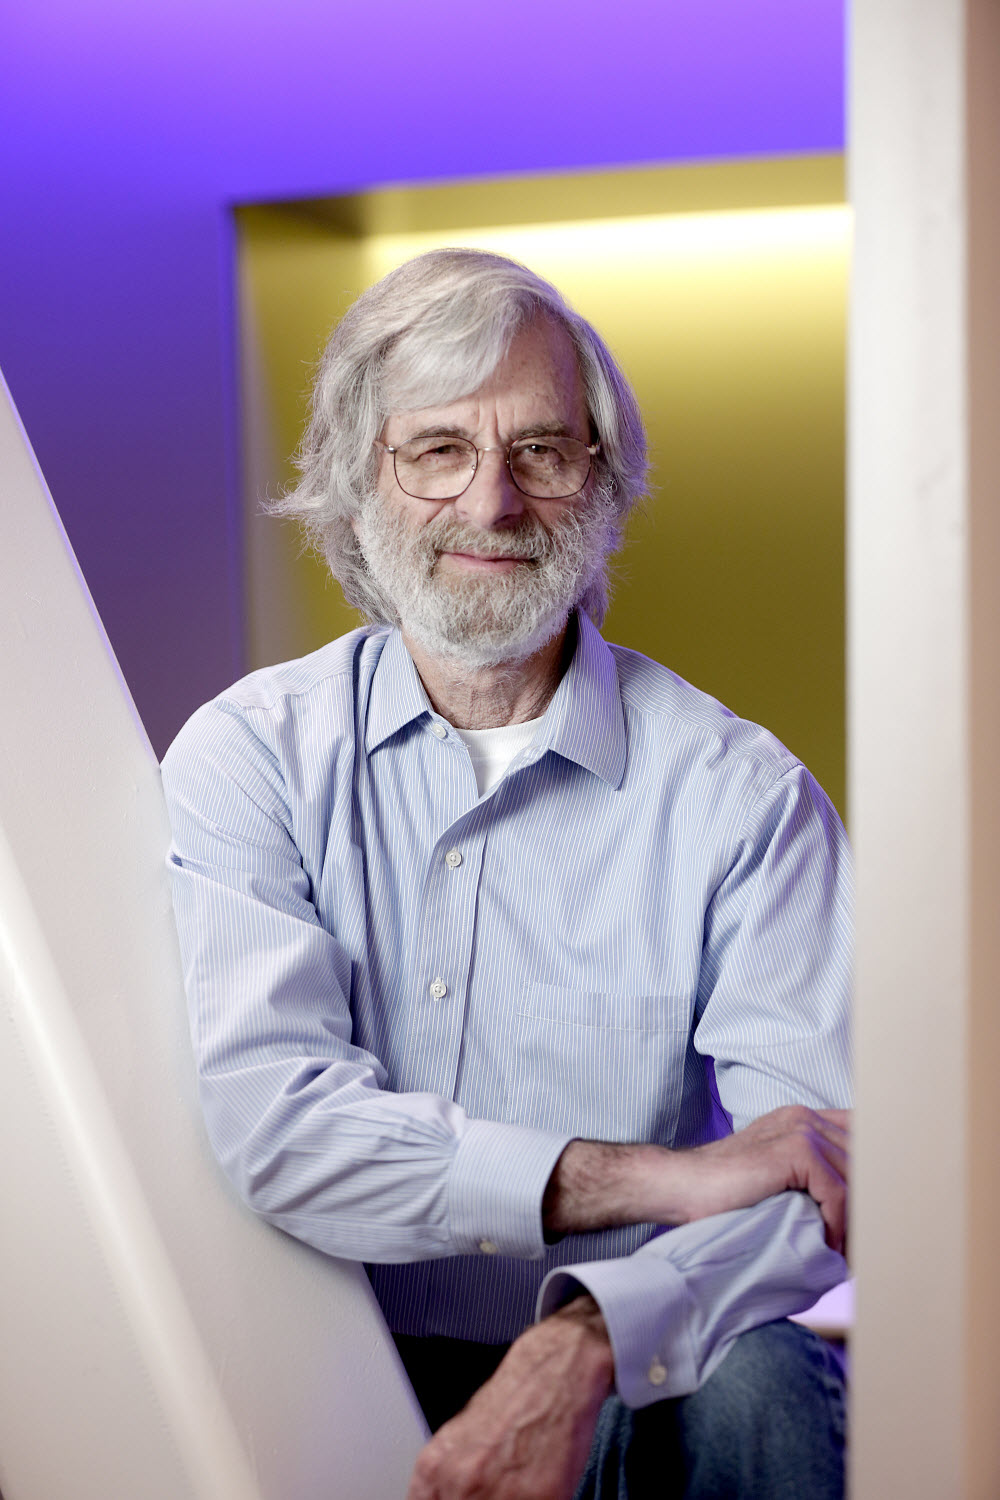
\includegraphics[scale=0.1]{./assets/lamport.jpg}
                    \caption{Leslie Lamport}
                }
            \end{figure}
        \end{column}
    \end{columns}

    \only<3>{
        \begin{figure}
            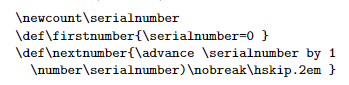
\includegraphics[scale=1]{./assets/plain-tex.png}
        \end{figure}
    }
\end{frame}

\begin{frame}{Core philosophy}

    \LaTeX{} core philosophy

    \begin{block}{\LaTeX}
        \begin{itemize}
            \item<1-> is free and open-source software
            \item<2-> provides professional levels of typesetting control
            \item<3-> produces the same output on any platform
            \item<4-> separates content from layout (`just start typing')
        \end{itemize}
    \end{block}

    \bigskip

    \only<5->{Still, there is quite a learning curve.}

    \medskip

    \only<6->{That is what this tutorial is for.}
\end{frame}

\begin{frame}{Creating a new document}
    \begin{columns}
        \begin{column}{0.5\textwidth}
            \begin{itemize}
                \item Visit Overleaf
                \item Click on ``Create a new project''
                \item Select ``Blank Project''
                \item Come up with a catchy title
                \item Hit `Create'!
            \end{itemize}
        \end{column}
        \begin{column}{0.5\textwidth}
            \begin{figure}[h]
                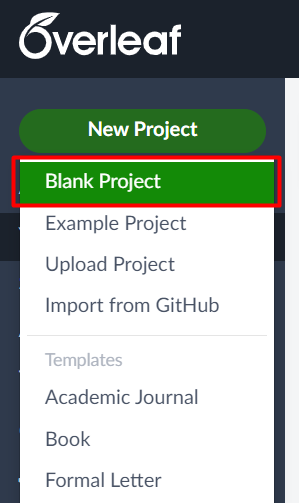
\includegraphics[scale=0.6]{./assets/new-project.png}
            \end{figure}
        \end{column}
    \end{columns}
\end{frame}

\begin{frame}{Overleaf}
    \begin{figure}[ht]
        \centering
        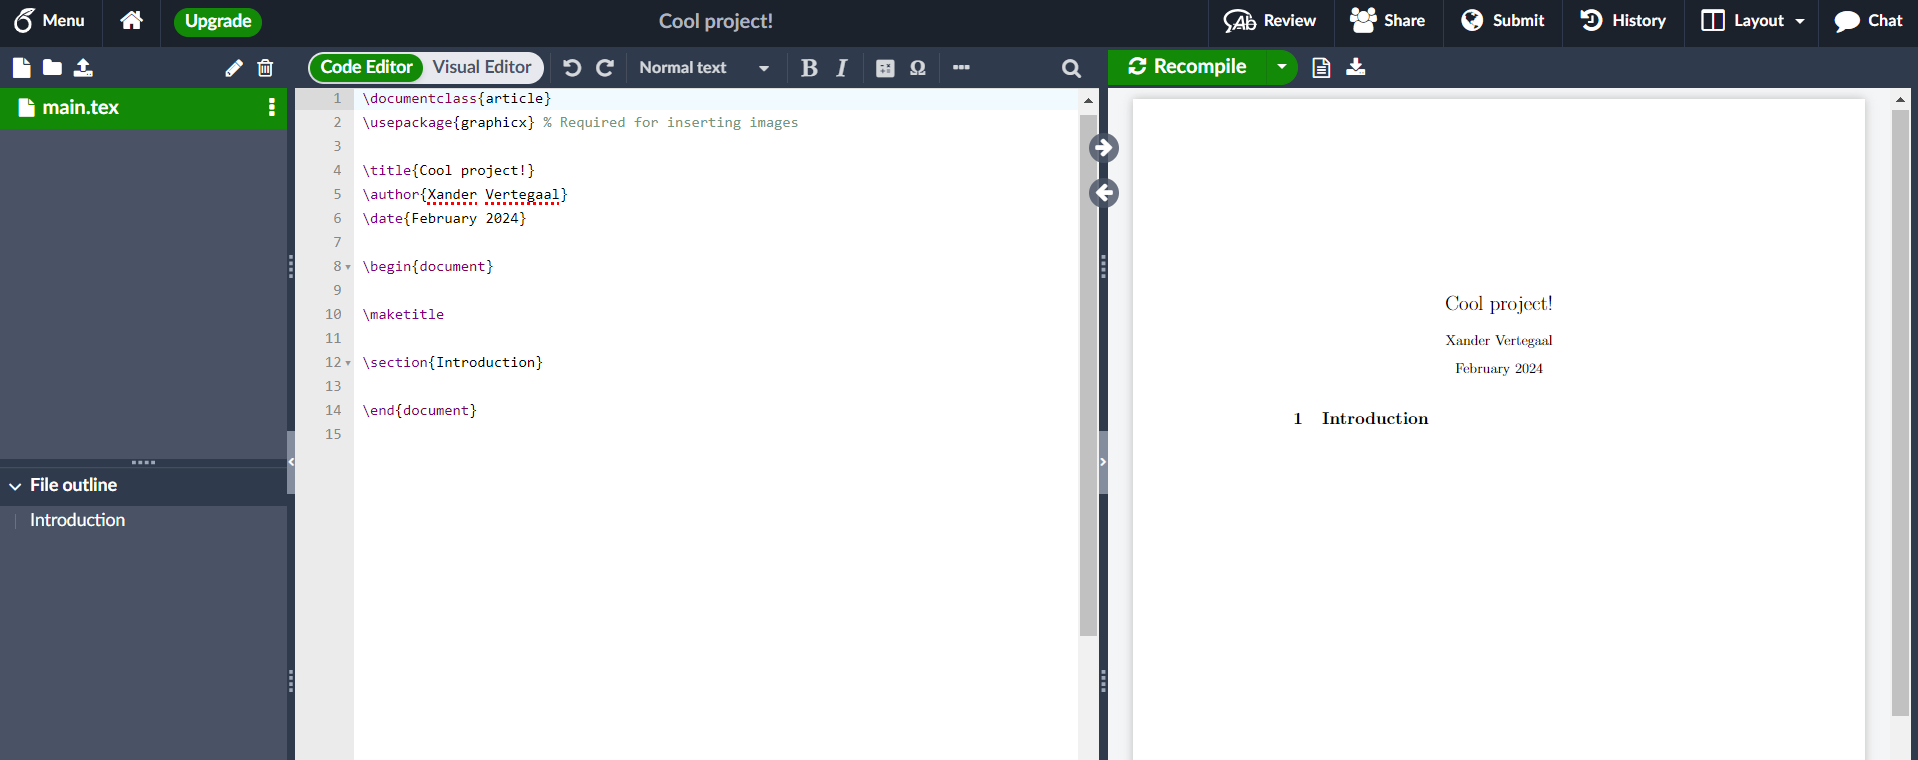
\includegraphics[width=\textwidth]{./assets/overleaf.png}
    \end{figure}
\end{frame}

\begin{frame}{\LaTeX{} commands}
    Simple commands (also called \textbf{switches}):
    \begin{center}
        \only<1>{
            \ttfamily
            \textbackslash{}maketitle

            \textbackslash{}LaTeX

            \switch{centering}
        }

        \only<2>{
            \ttfamily
            \red{\textbackslash}\blue{maketitle}

            \red{\textbackslash}\blue{LaTeX}

            \red{\textbackslash}\blue{centering}
        }

        \bigskip

        \only<2>{\red{backslash} + \blue{command name}}
    \end{center}
\end{frame}

\begin{frame}{\LaTeX{} commands}
    Commands with \textbf{mandatory} arguments:
    \begin{center}
        \only<1>{
            \begin{center}
                \ttfamily
                \textbackslash{}section\{Introduction\}

                \textbackslash{}author\{Albert Einstein\}
            \end{center}
        }

        \only<2>{
            \begin{center}
                \ttfamily
                \red{\textbackslash}\blue{section}\{\green{Introduction}\}

                \red{\textbackslash}\blue{author}\{\green{Albert Einstein}\}
            \end{center}
        }

        \bigskip

        \only<2>{\red{backslash} + \blue{command name} + \green{mandatory argument}}
    \end{center}
\end{frame}

\begin{frame}{\LaTeX{} commands}
    Commands with \textbf{optional} arguments:
    \begin{center}
        \only<1>{
            \begin{center}
                \ttfamily
                \textbackslash{}documentclass[12pt]\{article\}
            \end{center}
        }

        \only<2>{
            \begin{center}
                \ttfamily
                \red{\textbackslash}\blue{documentclass}[\purple{12pt}]\{\green{article}\}
            \end{center}
        }

        \bigskip

        \only<2>{\red{backslash} + \blue{command name} + \purple{optional argument} + \green{mandatory argument}}
    \end{center}
\end{frame}

\begin{frame}{\LaTeX{} commands}
    Environments:
    \begin{center}
        \only<1>{
            \ttfamily
            \textbackslash{}begin\{center\}

            \ldots

            \textbackslash{}end\{center\}
        }

        \only<2>{
            \ttfamily
            \red{\textbackslash}\blue{begin}\{\green{center}\}

            \ldots

            \red{\textbackslash}\blue{end}\{\green{center}\}
        }
        \sffamily

        \bigskip

        \only<2>{\red{backslash} + \blue{begin / end} + \green{environment name}}
    \end{center}
\end{frame}

\begin{frame}{Commands -- exercise}
    \begin{block}{Exercise}
        \begin{itemize}
            \item Type a few lines in the document body, and compile the document.
            \item Add a co-author to the \code{author} command with help of the \switch{and} \emph{switch}.
            \item Add another section to your document. Give it an interesting sounding name.
            \item Add an abstract to your document with the \code{abstract} \emph{environment}.
        \end{itemize}

    \end{block}
\end{frame}

\begin{frame}{Document structure}

    \only<1> {
        There are two required commands in a \LaTeX{} document:

        \begin{enumerate}
            \item the \command{documentclass}{\ldots} command;
                  \begin{itemize}
                      \item \code{article}: generic short(er) documents
                      \item \code{beamer}: for PPT-like presentations
                      \item \code{book}: full books
                      \item \code{letter}: letters
                      \item \code{report}: long articles with chapters
                  \end{itemize}
            \item a \latexenv{document} environment with some text.
        \end{enumerate}

        \medskip

        \begin{block}{Note}
            Document classes enable different layouts and commands. The \code{letter} class, for example, has a \command{signature}{\ldots} and a \command{closing}{\ldots} command.
        \end{block}
    }

    \only<2> {
        The document environment encapsulates the \textbf{document body}.

        \medskip

        Everything before that is called the \textbf{preamble}.

        \medskip

        This is where you do all of your initial configuration.
    }
\end{frame}

\section{Basic text formatting}
\begin{frame}{Typestyle (3.1)}

    \begin{table}[ht]
        \small
        \centering
        \begin{tabular}{rll}
            \toprule
            {\rmfamily\bfseries Effect}          & {\rmfamily\bfseries Command} & {\rmfamily\bfseries Switch} \\
            \midrule
            \textup{Upright shape}               & \command{textup}{...}        & \switch{upshape}            \\
            \textit{Italic shape}                & \command{textit}{...}        & \switch{itshape}            \\
            \textsl{Slanted shape}               & \command{textsl}{...}        & \switch{slshape}            \\
            \textsc{\rmfamily{}Small caps shape} & \command{textsc}{...}        & \switch{scshape}            \\
                                                 &                              &                             \\
            \textmd{Medium series}               & \command{textmd}{...}        & \switch{mdseries}           \\
            \textbf{Bold series}                 & \command{textbf}{...}        & \switch{bfseries}           \\
                                                 &                              &                             \\
            \textrm{Roman family}                & \command{textrm}{...}        & \switch{rmfamily}           \\
            \texttt{Typewriter family}           & \command{texttt}{...}        & \switch{ttfamily}           \\
            \textsf{Sans serif family}           & \command{textsf}{...}        & \switch{sffamily}           \\
            \bottomrule
        \end{tabular}
        \caption{Type styles with a sample text.}\label{tbltypestyle}
    \end{table}
\end{frame}

\begin{frame}{Typestyle (3.1)}
    \textbf{Usage}:

    \begin{center}
        This is upright. \textit{This is italic.} This is upright again.
    \end{center}

    \begin{enumerate}
        \item<only@1> With a \textbf{regular command}:

            \small\bigskip

            \texttt{This is upright. \command{textit}{This is italic.} This is upright again.}

        \item<only@2> With a \textbf{switch}:

            \small\bigskip

            \texttt{This is upright. \switch{itshape} This is italic. \switch{upshape} This is upright again.}

        \item<only@3> With a \textbf{scoped switch}:

            \small\bigskip

            \texttt{This is upright. \{\switch{itshape} This is italic.\} This is upright again.}

        \item<only@4> With an \textbf{environment}:

            \small\bigskip

            \begin{ttfamily}
                This is upright

                \command{begin}{itshape}

                \quad This is italic.

                \command{end}{itshape}

                This is upright again.
            \end{ttfamily}
    \end{enumerate}

\end{frame}

\begin{frame}{Typestyle -- Exercise}
    \begin{block}{Exercise}
        Create the following text in your document:

        \begin{itemize}
            \item \textbf{This is bold and sans-serif.}\hfill(Use regular commands)
            \item {\ttfamily This is upright and typewriter.}\hfill(Use switches)
            \item \begin{scshape}\rmfamily{}This is small caps.\end{scshape}\hfill(Use an environment)
        \end{itemize}
    \end{block}
\end{frame}

\begin{frame}{Text size (3.2)}
    \begin{table}[ht]
        \centering
        \begin{tabular}{rll}
            \toprule
            {\bfseries Effect}          & {\bfseries Command}         & {\bfseries Switch}    \\
            \midrule
            \Huge{Huge}                 & \command{Huge}{...}         & \switch{Huge}         \\
            \huge{huge}                 & \command{huge}{...}         & \switch{huge}         \\
            \LARGE{LARGE}               & \command{LARGE}{...}        & \switch{LARGE}        \\
            \Large{Large}               & \command{Large}{...}        & \switch{Large}        \\
            \large{large}               & \command{large}{...}        & \switch{large}        \\
            \normalsize{Normal}         & \command{normalsize}{...}   & \switch{normalsize}   \\
            \small{Small}               & \command{small}{...}        & \switch{small}        \\
            \footnotesize{Footnotesize} & \command{footnotesize}{...} & \switch{footnotesize} \\
            \scriptsize{Scriptsize}     & \command{scriptsize}{...}   & \switch{scriptsize}   \\
            \tiny{Tiny}                 & \command{tiny}{...}         & \switch{tiny}         \\
            \bottomrule
        \end{tabular}
        \caption{Text sizes with a sample text.}\label{tbltextsize}
    \end{table}
\end{frame}

\begin{frame}{Quotation marks (3.3)}
    \LaTeX{} does not automatically use opening and closing quotation marks.

    \medskip

    \begin{enumerate}
        \item For opening quotes, use \texttt{`}. \hfill (backtick, accent grave)
        \item For closing quotes, use \texttt{'}. \hfill (apostrophe, accent aigu)
        \item Double them for double quotes: \texttt{``} and \texttt{''}.
    \end{enumerate}

    \medskip

    \begin{center}
        \large
        \texttt{`Hello'} \textrightarrow{} `Hello'

        \texttt{``Hello''} \textrightarrow{} ``Hello''
    \end{center}
\end{frame}

\begin{frame}{Whitespace (3.5)}
    Note the following:
    \begin{itemize}
        \item \LaTeX{} ignores multiple spaces.
        \item \LaTeX{} ignores line breaks.
        \item \LaTeX{} ignores tabs.
    \end{itemize}

    \bigskip

    To create a new paragraph, use a blank line. For more vertical whitespace, use \switch{medskip}, \switch{bigskip}, or \switch{vspace} (see Section 3.5).

    \bigskip

    For horizontal whitespace, use \switch{quad}, \switch{qquad}, or \switch{hspace} (see Section 3.5).
\end{frame}

% \begin{frame}{Commenting (5)}
%     Use the \texttt{\%} sign to comment out text. The compiler will ignore it.

%     \bigskip

%     This can be convenient if you want to:

%     \medskip

%     \begin{itemize}
%         \item temporarily \emph{leave out} some text without deleting it;
%         \item add \emph{comments} to your document for collaborators;
%         \item \emph{speed up} the compilation process;
%         \item quickly find the source of a \emph{bug}.
%     \end{itemize}

%     \medskip

%     \begin{block}{Note}
%         Use Ctrl + / on Overleaf for quick commenting in and out.
%     \end{block}
% \end{frame}

\begin{frame}{Basic text formatting -- Exercise}

    \begin{block}{Exercise}
        Recreate the following text:

        \bigskip

        % hspace is needed to mimic the parindent in article style documents.
        \rmfamily
        \hspace{20pt}In the quiet town of \textsc{Willowbrook}, the villagers gathered on the market square to hear the royal messenger's proclamation: \textit{\Large``Hear ye, hear ye, citizens! The king has decreed that all citizens must wear a hat on Mondays!''}

        \medskip

        \hspace{20pt}\textbf{Rodney}, the village smith, started to look exceedingly worried and whispered to his wife: {\footnotesize``I don't own a hat.''}. \textbf{Eleanor}, careful not to raise attention, replied: {\footnotesize``Well, go buy one then!''}

        \medskip

        \hspace{20pt}``But it's Sunday!'' Rodney said.
    \end{block}
\end{frame}

\begin{frame}{Packages (intermezzo)}

    \textbf{Packages} are extensions to \LaTeX{} that provide additional functionality.

    \bigskip

    Import them in your \textbf{preamble} with the \command{usepackage}{\ldots} command.

    \bigskip

    That's it! You can now use the package's \textbf{commands} and \textbf{environments} in your document.

\end{frame}

\begin{frame}{Packages (intermezzo)}

    \begin{columns}
        \begin{column}{.5\textwidth}
            \only<1>{
                All packages are listed on CTAN, the \textbf{Comprehensive \TeX{} Archive Network} (\code{https://ctan.org}).
            }
            \only<2>{
                Almost every package has a \textbf{documentation} file. You can find it on CTAN or by typing \code{texdoc <packagename>} in your terminal.
            }
        \end{column}
        \begin{column}{.5\textwidth}
            \only<1>{
                \begin{figure}[b]
                    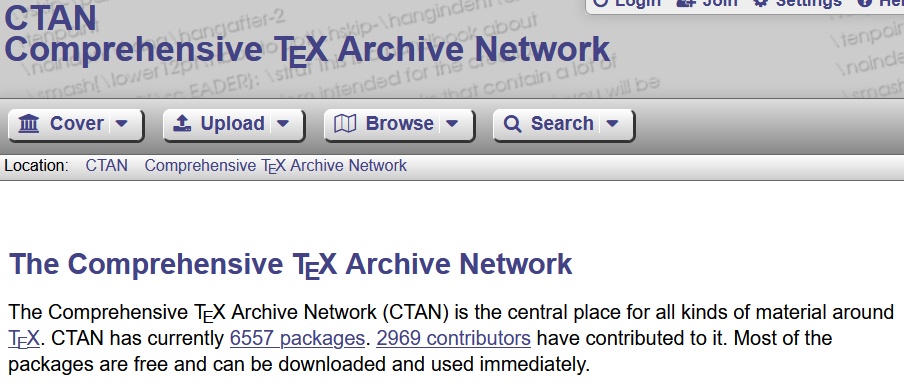
\includegraphics[scale=0.3]{./assets/ctan.png}
                \end{figure}
            }
            \only<2>{
                \begin{figure}[b]
                    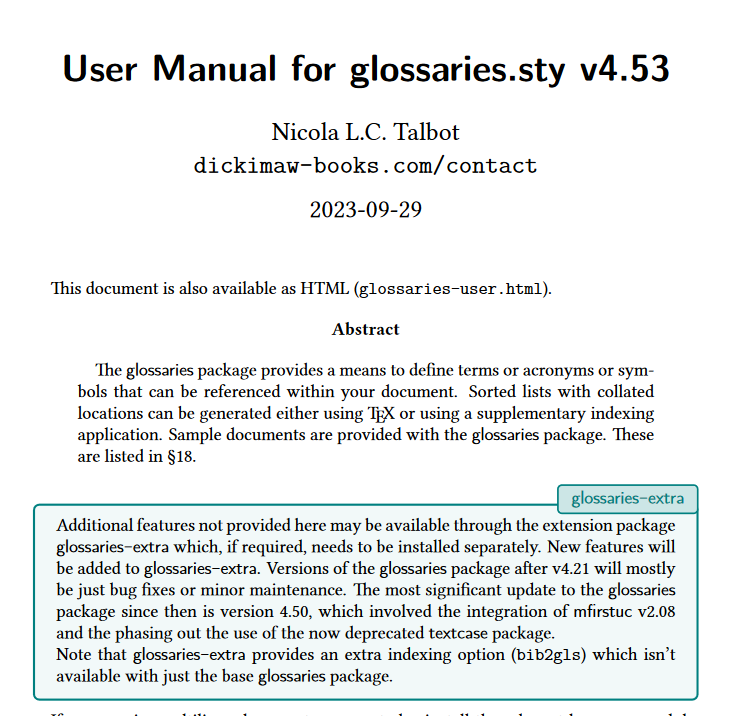
\includegraphics[scale=0.3]{./assets/ctan-doc.png}
                \end{figure}
            }
        \end{column}
    \end{columns}
\end{frame}

\begin{frame}{Changing fonts (3.7)}
    \LaTeX{} provides three built-in fonts:

    \medskip

    \begin{itemize}
        \item A main (serif) font:\hfill\textrm{Computer Modern}
        \item A sans-serif font:\hfill\textsf{Computer Modern Sans}
        \item A typewriter font:\hfill\texttt{Computer Modern Typewriter}
    \end{itemize}

    \medskip

    \only<2->{If you need more fonts, you need to import the \code{fontspec} package.}

    \medskip

    \only<3->{This requires the \hologo{XeLaTeX} compiler.

        \begin{center}
            \command{usepackage}{fontspec}
        \end{center}
    }
\end{frame}

\begin{frame}[fragile]{Changing fonts (3.7)}
    \only<1>{
        Option 1: \textbf{Override} one of the default font families:

        \bigskip

        \begin{itemize}
            \item \command{setmainfont}{Times New Roman}
            \item \command{setsansfont}{Comic Sans MS}
            \item \command{setmonofont}{Roboto Mono}
        \end{itemize}

        \bigskip

        Then use the familiar font commands (Section 3.1):

        \begin{itemize}
            \item \command{textrm}{\ldots} or \switch{rmfamily}
            \item \command{textsf}{\ldots} or \switch{sffamily}
            \item \command{texttt}{\ldots} or \switch{ttfamily}
        \end{itemize}
    }

    \only<2>{
        Option 2: \textbf{Create} a new font family:

        \bigskip

        \begin{center}
            \command{newfontfamily}{\textbackslash{}comic}\code{\{Comic Sans MS\}}
        \end{center}

        \bigskip

        Then use it with your own command:

        \begin{center}
            \ttfamily
            \{\textbackslash{}comic This is hilarious!\}

            \comic
            This is hilarious!
        \end{center}
    }

    \only<3->{
        Fonts are available:

        \bigskip

        \begin{itemize}
            \item as a \textbf{package} (URL in the handout)
            \item \textbf{preloaded} into Overleaf (URL in the handout)
            \item \textbf{installed} on your own system (not available on Overleaf)
            \item \textbf{uploaded font files} to Overleaf
        \end{itemize}
    }
\end{frame}

\begin{frame}{Changing fonts -- Exercise}
    \begin{block}{Exercise}
        \begin{itemize}
            \item Override your default sans-serif font and set it to {\arial{}Arial}.
            \item Create a new font family called \texttt{bettertimes} with the font {\bettertimes{}Times New Roman}.
            \item Find the `Gothic Textura Quadrata' font on the TUG Font Catalogue and use it in your document.
            \item {\minya Bonus: try to find this jolly font among the fonts listed in the Overleaf font overview.}
        \end{itemize}
    \end{block}
\end{frame}

\section{Lists}

\begin{frame}{Lists (7)}

    \LaTeX{} has three commonly used list styles:

    \bigskip

    1.\ \textbf{Unordered lists} (\code{itemize}):

    \begin{columns}[t]
        \begin{column}{0.5\textwidth}
            \begin{itemize}
                \item Apples
                \item Coffee
                \item Salami
                      \only<2->{
                          \begin{itemize}
                              \item Serrano
                              \item[€] Chorizo
                          \end{itemize}
                      }
            \end{itemize}
        \end{column}
        \begin{column}{0.5\textwidth}
            \ttfamily
            \command{begin}{itemize}

            \quad\switch{item} Apples

            \quad\switch{item} Coffee

            \quad\switch{item} Salami

            \only<2->{
                \quad\quad\command{begin}{itemize}

                \quad\quad\quad\switch{item} Serrano

                \quad\quad\quad\switch{item}[€] Chorizo

                \quad\quad\command{end}{itemize}
            }

            \command{end}{itemize}
        \end{column}
    \end{columns}
\end{frame}

\begin{frame}{Lists (7)}

    \LaTeX{} has three commonly used list styles:

    \bigskip

    2.\ \textbf{Ordered lists} (\code{enumerate}):

    \begin{columns}[t]
        \begin{column}{0.5\textwidth}
            \begin{enumerate}
                \item Apples
                \item Coffee
                \item Salami
                      \only<2->{
                          \begin{enumerate}
                              \item Serrano
                              \item Chorizo
                          \end{enumerate}
                      }
            \end{enumerate}
        \end{column}
        \begin{column}{0.5\textwidth}
            \ttfamily
            \command{begin}{enumerate}

            \quad\switch{item} Apples

            \quad\switch{item} Coffee

            \quad\switch{item} Salami

            \only<2->{
                \quad\quad\command{begin}{enumerate}

                \quad\quad\quad\switch{item} Serrano

                \quad\quad\quad\switch{item} Chorizo

                \quad\quad\command{end}{enumerate}
            }

            \command{end}{enumerate}
        \end{column}
    \end{columns}
\end{frame}

\begin{frame}{Lists (7)}

    \LaTeX{} has three commonly used list styles:

    \bigskip

    3.\ \textbf{Description lists} (\code{description}):

    \begin{columns}[t]
        \begin{column}{0.55\textwidth}
            \begin{description}
                \item[Apples] are delicious and it is said that they keep people with PhDs away.
                \item[Coffee] is a stimulant without which most academics would not survive.
                \item[Salami] is a type of sausage without which many Italians would not survive.
            \end{description}
        \end{column}
        \begin{column}{0.45\textwidth}
            \ttfamily
            \command{begin}{description}

            \quad\switch{item}[Apples] are \ldots

            \quad\switch{item}[Coffee] is a \ldots

            \quad\switch{item}[Salami] is a \ldots

            \command{end}{description}
        \end{column}
    \end{columns}
\end{frame}

\begin{frame}{Lists -- Exercise}
    \begin{block}{Exercise}
        Try to recreate the following list.

        \medskip

        My favourite fruits:

        \begin{enumerate}
            \item Bananas
            \item Mangoes
                  \begin{itemize}
                      \item[?] Are they in season?
                      \item[!] I don't know.
                  \end{itemize}
            \item Apples, esp. the following varieties:
                  \begin{description}
                      \item[Jonagolds] are nice and sweet.
                      \item[Granny Smiths] are very sour!
                  \end{description}
        \end{enumerate}
    \end{block}
\end{frame}

\section{Tables}

\begin{frame}{Tables (10)}
    \begin{table}[ht]
        \centering
        \begin{tabular}{|r|cl|}
            \hline
            Country     & Capital   & Inhabitants \\
            \hline
            Netherlands & Amsterdam & 17.02 M     \\
            Germany     & Berlin    & 82.67 M     \\
            \hline
        \end{tabular}
        \caption{A table about two countries.}
        \label{tbltables}
    \end{table}
\end{frame}

\begin{frame}[fragile]{Tables (10)}
    \small
    \begin{verbatim}
        \begin{table}[htbp]
            \centering
            \begin{tabular}{|r|cl|}
                \hline
                Country     & Capital   & Inhabitants \\
                \hline
                Netherlands & Amsterdam & 17.02 M     \\
                Germany     & Berlin    & 82.67 M     \\
                \hline
            \end{tabular}
            \caption{A table about two countries.}
            \label{tblcountries}
        \end{table}
        \end{verbatim}
\end{frame}

\begin{frame}{Tables -- Exercise}
    \begin{block}{Exercise}
        Recreate the following (right-aligned) table:
        \begin{table}[ht!]
            \flushright
            \begin{tabular}{r|l}
                \hline
                \textbf{Name} & \textbf{Inaugurated} \\\hline
                Barack Obama  & 2009                 \\
                Donald Trump  & 2017                 \\
                Joe Biden     & 2021                 \\\hline
            \end{tabular}
            \caption{US Presidents}
        \end{table}
    \end{block}
\end{frame}

\section{References}

\begin{frame}[fragile]{References (9)}

    Use \command{label}{\ldots} to label a section, figure, table or footnote.

    \medskip

    \begin{verbatim}
        \subsection{Analysis}\label{ssec:analysis}
    \end{verbatim}

\end{frame}

\begin{frame}[fragile]{References (9)}

    Use \command{ref}{\ldots} to refer to the number, or \command{pageref}{\ldots} to refer to the page.

    \medskip


    \small
    \begin{verbatim}
        As we saw in Subsection \ref{ssec:analysis} 
        on page \pageref{ssec:analysis}, the analysis
        is quite complex.
    \end{verbatim}
    \normalsize

    \begin{center}
        As we saw in Subsection \red{4} on page \red{17}, the analysis is quite complex.
    \end{center}

    \medskip

    When you add or remove subsections, these counters are automatically updated.

    \medskip

    Add the \code{hyperref} package to make your links clickable.

\end{frame}

\begin{frame}{References -- Exercise}
    \begin{block}{Exercise}
        \begin{enumerate}
            \item Add a label to the Introduction section in your document.
            \item Add a label to the table you created in the previous exercise. (Add it after the \code{caption}.)
            \item Refer to both your Introduction and your table in a new paragraph.
            \item Make sure that your references are clickable in the PDF.
        \end{enumerate}
    \end{block}
\end{frame}

\section{Bibliography}

\begin{frame}{Bibliography (11)}
    Setting up a bibliography in \LaTeX{} requires 5 steps.

    \medskip

    \begin{enumerate}
        \item Create a \filename{.bib} file.
        \item Add a reference to your \filename{.bib} file.
        \item Import the \texttt{biblatex} package and add your \filename{.bib} file to your preamble.
        \item Add a citation to your document.
        \item Print your bibliography.
    \end{enumerate}
    \bigskip
    We will be using \textsc{Bib}\LaTeX{} to manage our references.
\end{frame}

\begin{frame}{Bibliography}
    \textbf{Step one:} create a \filename{.bib} file.
    \medskip
    \centering
    \begin{figure}[hb]
        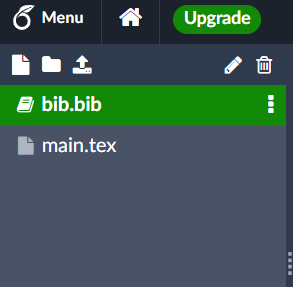
\includegraphics[scale=1]{./assets/bib.png}
    \end{figure}
\end{frame}

\begin{frame}[fragile]{Bibliography}
    \textbf{Step two:} add a reference to your \filename{.bib} file.

        {\centering\small
            \begin{verbatim}
        @article{lander1966counterexample,
            title={Counterexample to {E}uler’s 
              conjecture on sums of like powers},
            author={Lander, Leon J. and Parkin, 
              Thomas R. and others},
            journal={Bulletin of the American 
              Mathematical Society},
            volume={72},
            number={6},
            pages={1079},
            year={1966}
        }
    \end{verbatim}}

    \bigskip
    Tip 1: use Google Scholar to find \textsc{Bib}\TeX{} references.

    Tip 2: check the \textsc{Bib}\LaTeX{} package documentation for an overview of all fields.
\end{frame}

\begin{frame}[fragile]{Bibliography}
    \textbf{Step three:} import the \texttt{biblatex} package and add your \filename{.bib} file to your preamble.
    \medskip
    \centering
    \small
    \begin{verbatim}
        \usepackage[style=apa,backend=biber]{biblatex}
        \addbibresource{bib.bib}
    \end{verbatim}
\end{frame}

\begin{frame}[fragile]{Bibliography}
    \textbf{Step four:} add a citation to your document.

    Structure:

    \begin{verbatim}
        \cite[ pagenumbers ]{ citationkey }
    \end{verbatim}

    \begin{table}[ht]
        \centering
        \small
        \begin{tabular}{ll}
            \toprule
            \textbf{Command}                                  & \textbf{Result}                          \\
            \midrule
            \commandopt{cite}{lander\ldots{}example}{20}      & \cite[20]{lander1966counterexample}      \\
            \commandopt{parencite}{lander\ldots{}example}{20} & \parencite[20]{lander1966counterexample} \\
            \commandopt{footcite}{lander\ldots{}example}{20}  & \footnotemark                            \\
            \commandopt{textcite}{lander\ldots{}example}{20}  & \textcite[20]{lander1966counterexample}  \\
            \bottomrule
        \end{tabular}
        \caption{Citing commands}\label{tblcite}
    \end{table}
    \footnotetext{\cite[20]{lander1966counterexample}}
\end{frame}

\begin{frame}[fragile]{Bibliography}
    \textbf{Step 5:} print your bibliography.
    \medskip

    {\centering
        \begin{verbatim}
        \printbibliography
    \end{verbatim}}
    \printbibliography
\end{frame}

\begin{frame}{Bibliography -- Exercise}
    \begin{block}{Exercise}
        \begin{itemize}
            \item Go to Google Scholar and find a paper you wrote or one that you particular like.
            \item Export a \textsc{Bib}\TeX{} reference and place it in your \filename{.bib} file. (It might need to be cleaned up a bit.)
            \item Reference it in your text. Make sure it shows up in your bibliography.
            \item Now switch to the \code{authoryear} citing style.
            \item Bonus: use \command{citeyear}{\ldots}, \command{citetitle}{\ldots} and \command{citeauthor}{\ldots} to refer to the year, title and author of the paper, respectively.
        \end{itemize}
    \end{block}

    \bigskip

    If you have imported the \code{hyperref} package before, note that your references are now clickable!
\end{frame}

\section{Conclusion}

\begin{frame}{Use cases}

    \LaTeX{} has become the standard in the STEM sciences.

    \medskip

    It handles equations very well,

    \medskip
    {\rmfamily
        \begin{equation}
            \int_{-\infty}^{\infty} e^{-x^2} \cos(2\pi f x) \, dx = \frac{1}{2} \sqrt{\pi} e^{-\pi^2 f^2}
        \end{equation}
    }

    \medskip

    and graphs too.

    \medskip

    \begin{columns}
        \begin{column}{0.5\textwidth}
            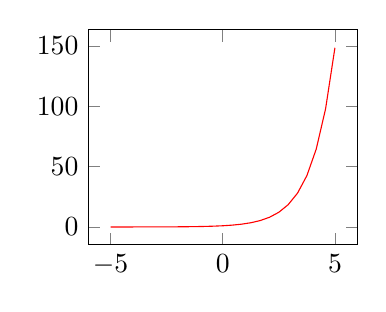
\begin{tikzpicture}
                \begin{axis}
                    \addplot[color=red]{exp(x)};
                \end{axis}
            \end{tikzpicture}
        \end{column}
        \begin{column}{0.5\textwidth}
            \ttfamily\small
            \command{begin}{tikzpicture}
            \quad\command{begin}{axis}
            \quad\quad\command{addplot}{[color=red]\{exp(x)\}}
            \quad\command{end}{axis}
            \command{end}{tikzpicture}
        \end{column}
    \end{columns}
\end{frame}

\begin{frame}{Use cases}

    But there is a lot more you can do with \LaTeX{}.

    \only<1>{
        \medskip
        Especially with the help of user-contributed packages.
    }

    \medskip\centering

    \only<2>{
        \begin{figure}
            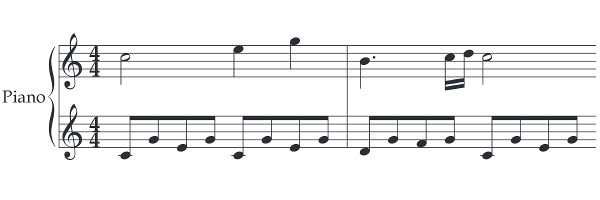
\includegraphics[width=.75\textwidth]{./assets/music.png}
            \caption{Musical notation (\code{musixtex})}
        \end{figure}
    }

    \only<3>{
        \begin{figure}
            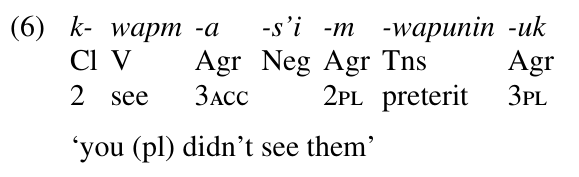
\includegraphics[width=.75\textwidth]{./assets/expex.png}
            \caption{Glossed and automatically numbered sentences (\code{expex})}
        \end{figure}
    }

    \only<4>{
        \begin{figure}
            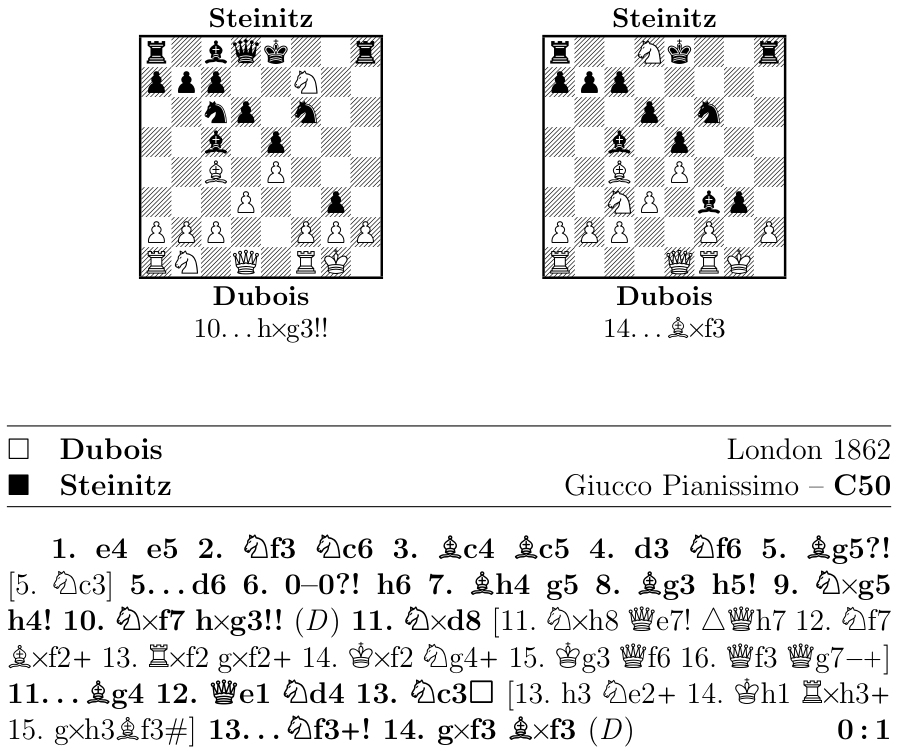
\includegraphics[width=.5\textwidth]{./assets/texmate-diagram.png}
            \caption{Chess notation diagrams (\code{skak} and \code{texmate})}
        \end{figure}
    }

    \only<5>{
        \begin{figure}
            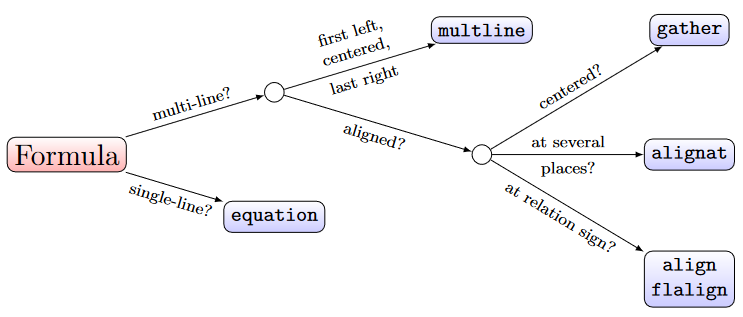
\includegraphics[width=.75\textwidth]{./assets/tikz-tree.png}
            \caption{Graphs (\code{tikz})}
        \end{figure}
    }

    \only<6>{
        \begin{figure}
            \begin{forest}
                [CP
                [C ]
                [TP
                [T ]
                [,phantom]
                [VoiceP, gray, tikz={\node [inner sep=5pt, fit to=tree] (pb) {};
                \draw[shorten <=20pt, shorten >=10pt, dashed] (pb.south west) .. controls (pb.north west) .. (pb.north east);}
                [Voice, gray]
                [\textit{v}P,gray
                [\textit{v},gray]
                [VP,gray
                [VP, roof, gray]
                ]]]]]
            \end{forest}
            \caption{Syntax trees (\code{forest})}
        \end{figure}
    }

    \only<7>{
        \begin{figure}
            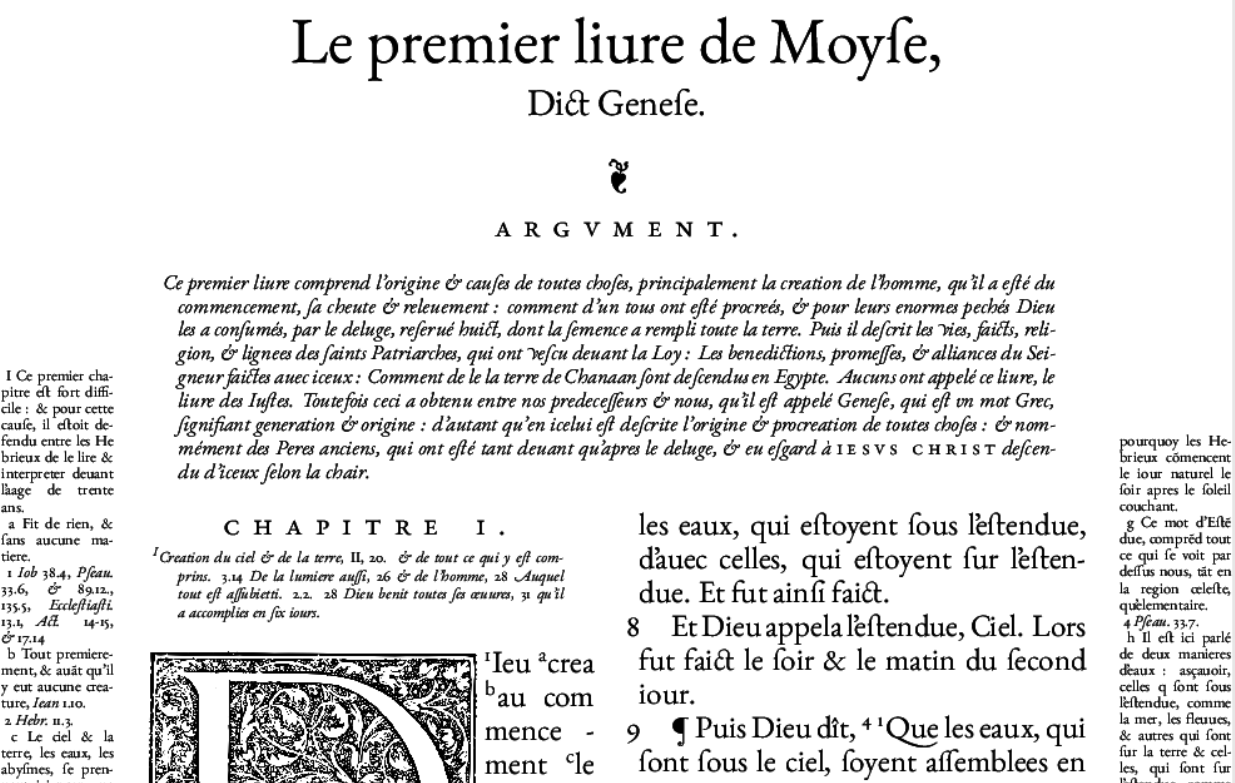
\includegraphics[width=\textwidth]{./assets/geneva.png}
            \caption{Facsimiles of manuscripts}
        \end{figure}
    }

\end{frame}

\begin{frame}{Use cases}

    But there is a lot more you can do with \LaTeX{}, also for non-academic purposes.

    \medskip

    \begin{enumerate}
        \item<2-> Curricula vitae
        \item<3-> Letters
        \item<4-> PowerPoint-like presentations
        \item<5-> Business cards
        \item<6-> Newsletters
        \item<7-> Books
    \end{enumerate}
\end{frame}

\begin{frame}{When (not) to use \LaTeX}

    \LaTeX{} is not always the best tool for the job.

    \bigskip


    \begin{columns}[t]
        \begin{column}{0.5\textwidth}
            \textbf{\LaTeX{} is great for:}
            \begin{itemize}
                \item<2-> scientific documents (articles, theses, books);
                \item<2-> official documents (letters, CVs, invoices);
                \item<2-> documents with complex typesetting requirements;
            \end{itemize}
        \end{column}
        \begin{column}{0.5\textwidth}
            \textbf{\LaTeX{} is not necessarily good for:}
            \begin{itemize}
                \item<3-> quick, private notes;
                \item<3-> presentations (\code{beamer});
                \item<3-> posters, flyers and other graphical documents;
            \end{itemize}
        \end{column}
    \end{columns}
\end{frame}

\begin{frame}{Troubleshooting}

    If you do not know how to do something in \LaTeX, you are likely not alone.

    \medskip

    \begin{itemize}
        \item Read \textbf{Overleaf}'s \LaTeX{} tutorial.
        \item \textbf{Google} your problem.
        \item Check \textbf{StackExchange}.
        \item Read the \textbf{package documentation}.
        \item Visit the Digital Humanities \textbf{walk-in hours} (this room, Thursdays, 14:00--15:00)
        \item Email us at the Research Software Lab.
    \end{itemize}

    \medskip

    \begin{figure}[ht]
        \centering
        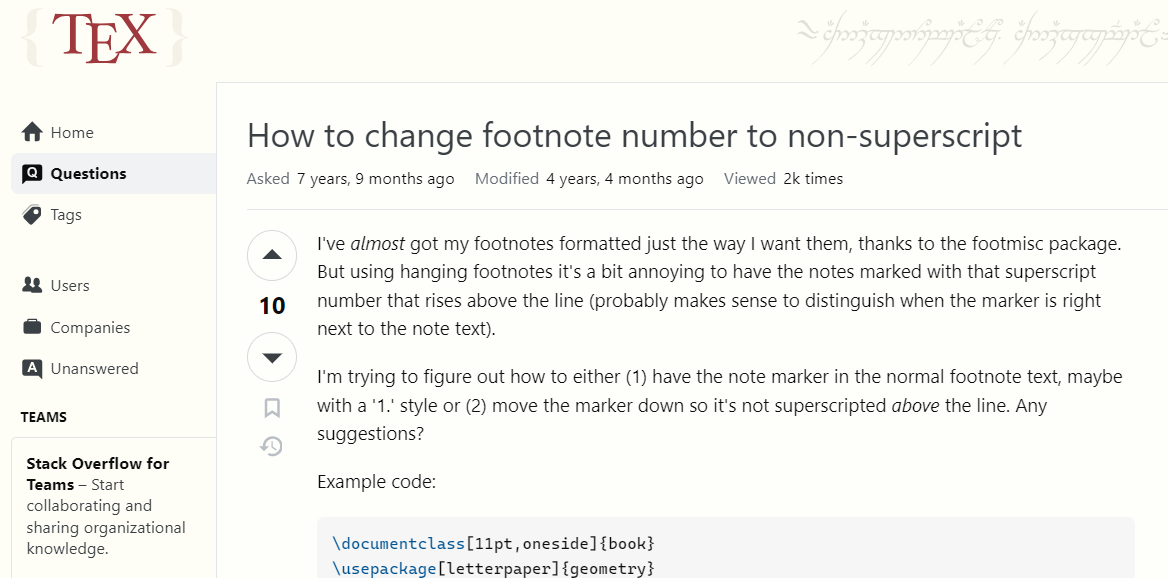
\includegraphics[width=0.5\textwidth]{./assets/stackexchange.png}
    \end{figure}

\end{frame}

\begin{frame}{Where to go from here}

    \LaTeX{} is a skill that needs practice to master.

    \medskip

    But it is a valuable tool for your academic and post-academic career.

    \medskip

    \begin{itemize}
        \item Rewrite an existing chapter/paper into \LaTeX.
        \item Write new non-urgent documents in \LaTeX.
        \item For new manuscripts: check with the editors first!
    \end{itemize}
\end{frame}

\begin{frame}{Thank you!}
    Thank you for your attention. I hope you have learned something useful today.
    \medskip
    \begin{center}
        \textit{Happy \LaTeX{}ing!}
    \end{center}
\end{frame}

\end{document}